% Made up for the tikra gallery: a matrix plot of 4 x 5 readings, shaded between its cells.
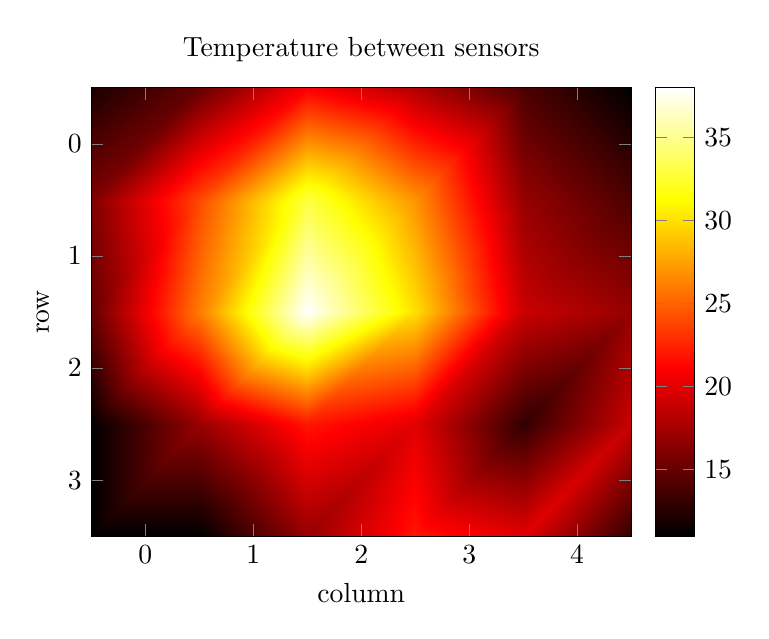
\begin{tikzpicture}
\begin{axis}[view={0}{90}, colormap/hot2, colorbar, enlargelimits=false,
    title={Temperature between sensors}, xlabel=column, ylabel=row]
  \addplot[matrix plot, shader=interp, mesh/cols=5, point meta=explicit] coordinates {
    (0,0) [12] (1,0) [15] (2,0) [21] (3,0) [18] (4,0) [14]
    (0,1) [16] (1,1) [24] (2,1) [33] (3,1) [27] (4,1) [17]
    (0,2) [15] (1,2) [26] (2,2) [38] (3,2) [30] (4,2) [19]
    (0,3) [11] (1,3) [17] (2,3) [22] (3,3) [20] (4,3) [13]
  };
\end{axis}
\end{tikzpicture}
